%! Ian Melnick
%! 04-25-06 
%! Spinelli, Hemmendinger
%! CSC-295H Sophomore Independent Research 


\documentclass[12pt,letterpaper,titlepage]{article}   % ,twoside
\usepackage[pdftex]{graphicx}
\usepackage{apacite,geometry,fancyhdr,setspace,url,wrapfig,lgrind,verbatim}
\geometry{margin=1in}
\headheight 15pt

\title{CampusQuest\\
  {\small Exploring Graph Theory and the Shortest Route Problem in Java}}
\author{Ian Melnick}
\date{May 5, 2006}


\begin{document}
\maketitle
\begin{spacing}{0.9}
\tableofcontents
\end{spacing}

\newpage
\pagestyle{fancy} %headings
\doublespacing


\section{Abstract}

A Java application was created to use Dijkstra's shortest path algorithm
to determine the best route between any two locations in the Science and
Engineering Complex. Output resembles online driving direction services
like MapQuest. A user selects start and destination rooms, and is
provided with a map outlining the best walking path. Text-based
turn-by-turn directions are additionally provided, and include estimated
travel distance. The program works both stand-alone and as a web browser
applet, and can accommodate other buildings and outdoor locations on
campus. To allow for ease of expansion, a built-in graphical interface
is included to provide new maps and label significant points. Distances
are calculated automatically based on map scale size, but manual
distance specification is also possible for special cases like
stairwells and elevators.


\section{Acknowledgements}

Maps for this project were provided by Loren Rucinski and Fred Puliafico
of the Union College Facilities Services Department. Special thanks to
David Hemmendinger and John Spinelli for their guidance and support.


\newpage
\section{Introduction and Background}

This project's objective is to create path-finding software that would
allow guests, students and faculty to more easily navigate the buildings
on Union's campus. Users would be able to select starting and
destination points, and the program would return step-by-step
instructions. Like the driving directions service at \emph{MapQuest.com}, a
graphical route would also be displayed. Ideally, the directions
determined by the software would be the shortest possible walkable route
between the two locations.

Finding the shortest route is a lengthy task. For a person, determining
the shortest route between two places requires the discovery of every
possible way of getting to the destination. Determining a single valid
route may enough of a challenge. Then the distances for each of the
routes must be measured, and conclusions are drawn. In a very large
environment, this process can become so time consuming that it may be
realistically impossible to complete. When employing a computer, the
process works similarly, only the computer has the advantage of knowing
where every reachable location is from the start. With this knowledge,
the shortest route can be found much faster---it's simply a matter of
determining the relationships between all the available locations.

A lot of modern technology exists to help people more easily navigate
the world around them. As mentioned earlier, online services like
\emph{MapQuest.com} and \emph{Google Maps} provide driving directions
services for
most parts of the United States. This allows people to quickly find out
how to get somewhere without guessing or using a paper map. Typically in
these web-based services, a user inputs the starting and destination
locations, and the website returns text-based turn-by-turn directions
and a map depicting a graphical route. Also common in the modern
navigation technologies are \emph{Global Positioning System} devices. These GPS
units use satellite signals to determine where a person is situated on
the Earth. GPS has become so common and advanced that it is now
available both in cars and as handheld units. Like the online services,
GPS are able to provide outdoor driving and walking directions.

Nearly all the technologies that deal with displaying and using
geographical data use special software known as a \emph{Geographic Information
System}. A GIS is a sophisticated database that, in simplest terms,
describes where things are and what they look like. They can be used to
input and display roads and rivers, demographics and trends, and
practically any other geographically-related information. While this
project does not employ such advanced technology, it does implement
basic concepts found in these systems to meet the project objectives.
\cite{wiki:gis}

Perhaps the most important aspect in a computer-driven geographic system
is the way in which information is represented internally. Data must be
stored in such a way that it can both be accessed and manipulated by the
computer, and be translated into a visual representation for the user.
Additionally, systems that represent many different kinds of data must
be able to correctly relate them together. A simple example is relating
the physical geographic information to the specific data associated with
it. Geographic data may be stored as a typical raster image (i.e., a
JPEG), and descriptive data (such as city names) is stored in a separate
location. The descriptive data must contain information that describes
where it exists relative to the map image, such that it can be
superimposed correctly. Think about drawing city names on a map---if the
locations of where the names belong are unknown, the names are
meaningless. The more complex alternative is a ``vector'' format, where
information describing the geographic data is stored, rather than the
image itself. This makes it easier for large-scale GIS systems to
accurately depict data and internally relate many types of information
together. Rather than having to draw metadata on top of an image, the
metadata can be drawn within the image. \cite{wiki:gis}

For this project, emphasis is placed most on determining shortest routes
within buildings. Therefore, a simple raster-based map works fine for
representing floor plans, with descriptive (route) information being
superimposed. This allows the data representation mechanism to be
focused solely around the project objectives. In this case, a location
can simply be considered a coordinate on a map. The path connecting the
locations can simply be a line.

In computer science, the graph data type fits this requirement
perfectly. A graph consists of nodes (a.k.a points, vertices) and edges
(lines), and unlike a tree, a graph has no defined structure to conform
to. This allows a graph to be used for representing locations and the
paths that connect them. Graphs are so often used for this purpose that
the study of this topic has a name---graph theory. Of course, graphs are
not limited to geographical modeling, and also are commonly used for
describing computer networks. Various properties can be applied to edges
to make the network model more meaningful. For example, edges that have
an assigned length are known as weighted edges, and a graph with
weighted edges is
known as a weighted graph. Weighted edges are useful
for indicating distance between points. In certain cases, a path may
only be valid in one direction---think of a one-way street. This
property is known as directed edges, and a graph that is made of
directed edges is called a directed graph. Similarly, a graph which does
not have directed edges is called an undirected graph. Weighted and
directed edges can be combined to represent complicated networks.
\cite{wiki:gt}

Normally, a program must do more than simply store a graph---most
applications require the ability to step through it in a meaningful
order. Graph traversal is the process of ``walking'' from node to node
via the edges. Common traversal techniques include breadth-first search
(BFS) and depth-first search (DFS). Topological sort, though a sorting
technique, can also be considered a traversal method since it walks from
node to node within the graph. This approach requires a directed graph,
and nodes are traversed based on what other nodes point to them. The
breadth- and depth-first searches require neither weighted nor directed
graphs. Think of a depth-first search as the process of exploring the
length of a corridor without attempting to visit every single room along
the way, coming back to the passed-by rooms later. A breadth-first
search is the opposite---visiting each nearby room before advancing
further down the corridor.

A simple graph traversal will not solve the shortest path problem on its
own. Single-source shortest path algorithms like Bellman-Ford and
Dijkstra use these traversal methods to determine the shortest paths
between two points. The shortest route also may not always be the
fastest route, and in this report, whenever ``best route'' is used, it
is used to mean ``shortest route''. The strengths and weaknesses of
these various algorithms will be discussed later, but keep in mind that
Dijkstra's algorithm, a BFS-based solution, is key to reaching the
project's goal. 

Though it may not be powerful enough to compete with online driving
directions services, this project is still quite useful. It has the
potential to be another item in Union College's toolbox of things to
make visitors' lives easier. The project is able to support any building
on campus and any outdoor area, provided basic floor plans are
available. Though the Science and Engineering Complex has been used as a
proof-of-concept, the program has the potential to extend to the entire
campus, and provide a truly useful service to the Union community. It
could also be used in malls, Chicago's McCormick Place, or other large
areas where an interactive map would be useful. Additionally, it could
be used within other similar projects to make an even more powerful
tool. The disadvantage to these types of technologies, however, is that
people become less dependent on directional instincts and more dependent
on potentially buggy software and outdated maps. Most companies pride
themselves however on map accuracy, and overall, the ability to be able
to get immediate directions is really priceless. 

The remainder of the report will discuss project-specific requirements,
alternatives chosen for the implementation, and a detailed description
of the implementation itself. A program user's guide and maintenance
manual is also included at the end.


\section{Design Requirements}

The program needs to be able to present a graphical interface that would
allow the user to specify start and destination points. This display
would include a map of the current floor (within the current building),
which can be panned using the mouse. Available locations would be drawn
on top of the map. Both text-based step-by-step directions and an
outlined graphical route must be returned. As the user steps through the
given directions, the map should update to display the currently
described position.

To prepare the program for use, the maintainer must obtain floor plans
of the building and manually specify accessible locations and their
relationships. This data entry should be performed through a similar
graphical interface, in which the input is achieved via click-and-drag.

The program must be able to write the location information to a file,
and be able to read the JPEG image format for floor map display. An
appropriate shortest path algorithm must be implemented to determine the
best route between two points. This need not be the fastest route as
well; therefore, tracking time between points is not a requirement, but
an option. The route-finding logic must be able to function between
multiple floors, and be designed such that obtaining routes between
buildings is also possible. To avoid over-complexity in the first
version of the software, accommodations for special needs is not
required. This primarily involves users who are limited to elevator use
for travel between floors. 


\section{Design Alternatives}

Java is an appropriate programming language choice, as it is
write-once-run-anywhere, and thus very portable. It also can be used to
create stand-alone applications as well as ``applets'' that are executed
via a web browser. Additionally, by using a language that is widely used
and well-known, the potential for ability to integrate the software into
other future projects increases. Java 1.5 (JDK 5.0) is the most recent
public release of the language, and it includes new features like
generics and autoboxing which were useful for development. Since it is
backwards-compatible with older Java conventions, it made sense to
develop the project using JDK 5.0.

Though I considered using the Java OpenGL graphics libraries for
rendering output, they introduce another variable in the development
process. OpenGL would need to be studied and learned, and could impede
development of the primary components. Since the standard Java AWT
library meets the needs of the project, it was chosen for use.
Similarly, Java's built-in windowing toolkit (Swing/AWT) was chosen for
building the interactive components, since it is powerful enough for the
requirements of the project.

Serializing the graph data to an XML-based storage format would allow
certain data to be modified using a text editor. Beginning with Java
1.4, a built-in XML object encoder/decoder has been offered through the
java.beans package. However, it is limited as to what kinds of objects
it can serialize, and it was found during testing that it is unreliable
for serializing linked data structures. Free third-party XML
serialization libraries are available, such as Xstream, XMLWriter and
XOM. In terms of usage, these libraries do not quite function the same
way as Sun's built-in serialization techniques. If in the future a
different serialization format was desired (or these libraries had
unforeseen problems), much code would need to be modified to adapt to
the change. While a wrapper class could be produced to allow for an easy
transition, it was again decided to focus more on the development of the
primary functional components. Therefore, Java's traditional object
serialization strategy was chosen, regardless that it is a binary
format. Though minor data touch-ups will be impossible, it does force
the data entry/editing portion of the project to be fully functional.

The program must be able to represent specific locations as well as the
paths between them. A graph type data structure fits this requirement
very well. In a building, paths between any two points are always
positive, and have constant distance. Therefore, the data can be
represented using an undirected, positively-weighted graph. While Java
provides many different abstract data types, a Graph class was not found
in the Java 1.5.0 class library. Therefore, it was decided that a
graph-like class would be created and tailored to meet the specific
requirements of the project. Array-based storage for a very large number
of elements might become inefficient if/when dynamic resizing is
necessary. And if a classic two-dimensional array is used to represent
the graph, given the graphs are undirected, this would introduce large
space inefficiency as well. Therefore, nodes and edges will be stored
using linked lists. 

Of the three common shortest path algorithms, Dijkstra's algorithm is
the best fit. All paths in any building have a positive distance, so the
Bellman-Ford algorithm is unneeded. Floyd-Warshall is also ruled out
since the shortest route is required between only two specific points at
any given time. Since the project's specifications do not include any
caching method for route results, algorithm efficiency is also
important. Therefore, Dijkstra's algorithm was chosen. \cite{skiena}


\section{Final Design and Implementation}

I wrote the software in Java 1.5, using Dijkstra's shortest path
algorithm for determining routes. Java's AWT libraries were used for
graphical display, and the built-in object stream methods were used for
storing and retrieving graph data. First I'll describe how the program
operates, and later provide a more detailed explanation of its classes.

Application mode, map, and screen dimensions are specified via
commandline arguments or applet parameters. If no arguments are
provided, default settings are assumed. Available modes are ``Editor''
and ``Router'', where the former provides a data entry environment, and
the latter is the end-user route finding interface. In both modes, a map
of the requested floor is drawn in a window, with directional
information drawn on top of it. The editing mode is used to store this
information, while the routing mode uses this data to show the user
where to go. 

Locations are represented by ``nodes'' which store coordinates relative
to a certain position on the map. Accessible nodes are represented by
green circles, while invisible nodes are represented by yellow circles
(editing mode only). Invisible nodes are used for corners, turns and
other locations which are not significant destinations. They are
necessary in order to provide an accurate description of a walking path.
Each node contains a list of ``edges'', or paths, that it is directly
connected to. Therefore, relationships between nodes are determined by
edges that nodes have in common. On the map, edges are displayed with
black lines. The program automatically determines edge length by
calculating the distance between the nodes it relates. By using the
screen and print resolutions of the base map image, the program is able
to report these distances in terms of feet.

Since the map is very large, only a portion of it is displayed on the
screen at any given time. It can be panned using click-and-drag and
mouse wheel scrolling. Clicking the mouse wheel changes scroll
direction. In editing mode, the map's position can also be manipulated
using sliders.

Routing mode provides the user with drop-down menus that list source and
destination rooms. When valid locations are selected, a text box with a
list of directions is returned. Next and previous buttons are provided
at the top of this window. Within the list, the current position shown
on the map is indicated using arrows. As the user clicks through the
list, the map centers itself around the currently described position.
This makes it easy for the user to see where to go. If the next position
involves a different floor, the current map is replaced with the
appropriate one.

In editing mode, the maintainer may create nodes by double-clicking over
the position of the desired spot. A node may be moved by clicking and
dragging it to a new location. Edges are created by clicking and
dragging from one node to another. A menu for modifying a node is
provided when the node is double-clicked on. This menu allows the
maintainer to change the node's description, modify its edges, and link
it to other floors. Typically, only nodes representing stairwells and
elevators are linked to other floors. Changes to the graph are saved
using the Save button, and are loaded via the Load button.

Saving to and loading from different configuration files is not
supported; the graph data is saved to a DAT file with the same file name
as the respective map image. Graph data files are saved to and loaded
from the home directory of the current user. Map images must follow a
specific naming convention: map\_building\_floor.jpg, where building
specifies the building, and floor specifies the floor. Note that png-
and gif-format map images are also permissible, though only jpg-type
images have been used for this project.

There are thirteen public classes: \texttt{Main}, \texttt{Editor}, 
\texttt{Router}, \texttt{MapComponent}, \texttt{MapItem}, 
\texttt{NodeItem}, \texttt{EdgeItem}, \texttt{Dijkstra}, 
\texttt{NodeEditor}, \texttt{FloorLinker}, \texttt{DirectionsFrame},
\texttt{Utility} and \texttt{Errors}.

\subsection{Main, Editor and Router}

\texttt{Main} is responsible for launching the program. It extends
\texttt{javax.swing.JApplet} so that it can be run directly as an applet, or
encapsulated within a \texttt{JFrame} for stand-alone operation. It calls
\texttt{Utility.getArgs} to parse the parameters sent to the program either via
commandline or HTML. Bruce Eckel's Console class is used for the
applet-to-frame encapsulation. \cite{tij}

\texttt{Editor} and \texttt{Router} are the two main interactive classes,
and are in
charge of running the rest of the program. Only one is used at a time.
They each set up the appropriate windowing environment, and contain
specific callback methods that are invoked when the user performs an
action. For example, all click and drag-and-drop functionality is
defined in \texttt{Editor}'s \texttt{MouseMethods} class. When the mouse
is clicked,
\texttt{mouseClicked()} is called. If the first or third mouse buttons have been
double-clicked over an empty space, a new node is created there; if a
double-click occurs over an existing node, the \texttt{NodeEditor} is called on
it. As another example, \texttt{mouseReleased()} is called whenever a mouse
button has been released. It checks to make sure that the mouse was
dragged first, and then does one of three things: move a node, create an
edge, or move the map. All of the callback functions extend or implement
Java's mouse-action classes.

\texttt{Router} has similar mouse and button-related callback functions, though
they're not as complex as \texttt{Editor}'s. \texttt{Router} is mostly 
concerned with
properly displaying menus that allow the user to select start and
destination locations. The \texttt{setNodeList()} method is used to generate a
list of all possible places from every available map, and this list is
later loaded into the \texttt{JComboBox} menus that the user selects from. The
\texttt{setMap()} and \texttt{update()} methods are used to set and display 
\texttt{Router}'s map
component, so that different maps can be loaded within the same session.
This is required when traveling between multiple floors. Management of
the map itself, however, is left to the \texttt{MapComponent} class.

\subsection{MapComponent}

\texttt{MapComponent} is responsible for handling and displaying all map-related
graphical information. This includes drawing the base map as well as the
nodes and edges on top of it. As a \texttt{JComponent}, \texttt{MapComponent}
can be used
in any Swing application, and is completely self-contained. The
\texttt{paintComponent()} method is called by Java every time a
\texttt{JComponent} needs to
be rendered. Therefore, the main display logic for the 
\texttt{MapComponent}
resides within this method. The base map is opened as an  \texttt{ImageIcon},
which is then painted on to the \texttt{MapComponent}.

Again, since the map image is larger than the available screen area, not
all of the map can be shown at once. Panning occurs by shifting the
painted location of the \texttt{ImageIcon}. Experiments with these painting
routines found that Java considers the top-left corner of the component
as the origin, with the bottom-right corner being the maximum. This is
illustrated in Figure \ref{coordsdiag}. Painting of the image begins at
the origin of the component. Therefore, to view
image area beyond the boundaries of the component, the image must be
shifted upwards and leftwards. This forces the origin of the painted
image to be negative relative to the origin of the component.
Thus, when drawing the map, coordinates are nearly always negative.

%\begin{wrapfigure}{r}{75mm}
\begin{figure}
\begin{center}
  \scalebox{0.5}[0.5]{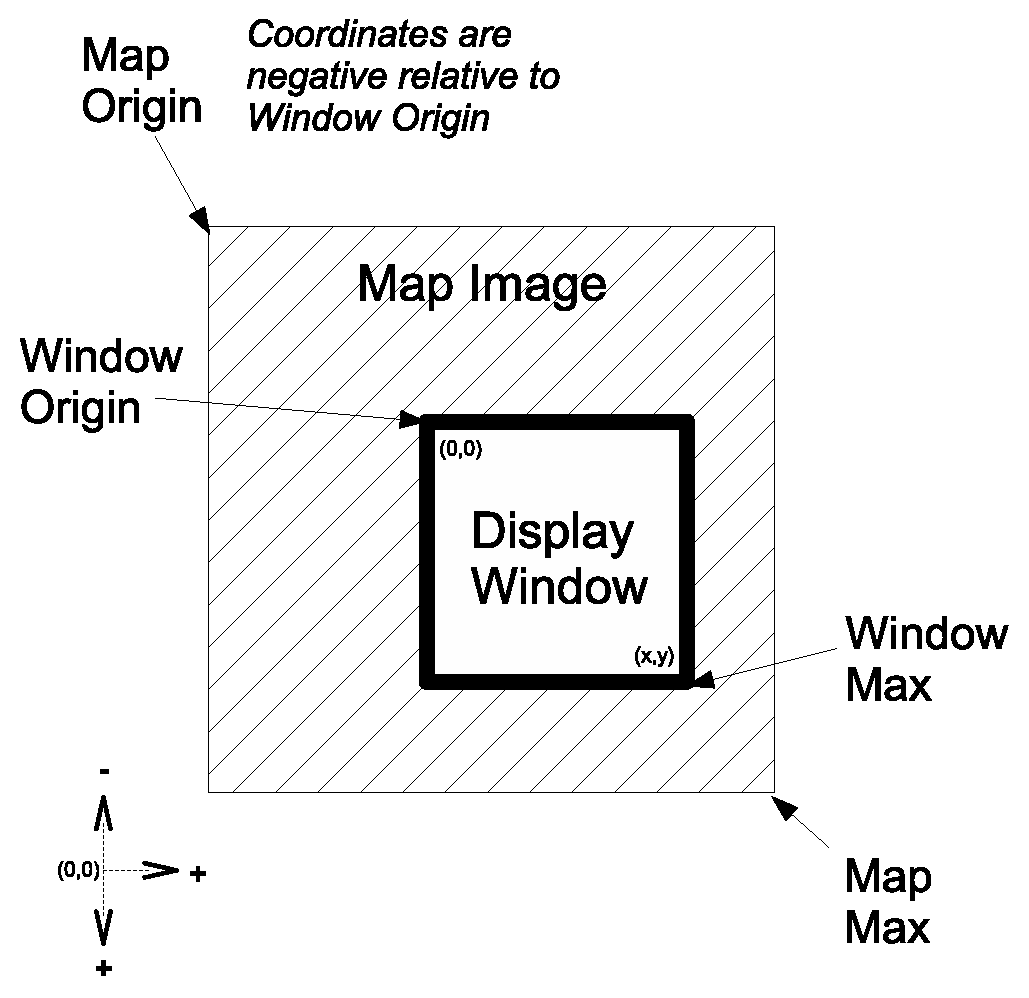
\includegraphics{images/pdf/map-coords-diagram}}
\end{center}
\caption{Map Coordinates Diagram}
\label{coordsdiag}
\end{figure}
%\end{wrapfigure}

When the component becomes mouse-aware, coordinate issues are further
complicated. Mouse coordinates are always positive, as they are relative
to the component, and only apply within the component's boundaries. In
other words, two coordinate systems are used within the
\texttt{MapComponent}---one that specifies the origin of the map, and the other
that tracks the location of the mouse. The former always is a negative
pair, while the latter is always a positive pair. Therefore, the
MapManager class deals with map manipulation, and map-mouse
relationships.

Some examples of methods found in \texttt{MapManager} are
\texttt{centerAroundPoint()} and \texttt{mouseCoordsToMapCoords()}.
The former is designed
to center the map on a point relative to the visible component. The
latter converts mouse coordinates (relative to component) to the
appropriate location on the map.

Originally the methods contained in \texttt{MapManager} were simply methods of
\texttt{MapComponent}. However, \texttt{MapComponent} is also responsible
for drawing
nodes and edges. Early on, node management methods were also plain
methods of \texttt{MapComponent}. Later, the map-related and
node-related methods
were separated, to allow \texttt{MapComponent} to be more easily
understood and maintained. Thus, \texttt{MapComponent} contains another
class of helper methods,
called \texttt{NodeManager}. \texttt{NodeManager} is essentially the specialized
graph-like class that was discussed in the previous section. Anything
related to node manipulation is performed through it. \texttt{NodeManager}
deals with storing nodes, tracking their relationships, and saving and loading
this data to and from a file. Like \texttt{MapManager}, however, 
\texttt{NodeManager} depends on the \texttt{MapComponent} 
environment---it is a part of \texttt{MapComponent}'s
core functionality---and therefore, it is inappropriate to separate
\texttt{NodeManager} into an entirely separate class.

The \texttt{MapComponent.initMap()} method exists to allow for the
\texttt{NodeManager}
data to be accessible without loading the respective map image. While
most cases require both the map and nodes to be loaded simultaneously,
in certain situations, it is only appropriate to load the node data.
More on this later.

\subsection{MapItem, NodeItem and EdgeItem}

While \texttt{NodeManager} should be considered the graph-like data structure,
the data objects it stores are \texttt{NodeItem}s. Therefore, 
the \texttt{NodeItem} class
represents nodes on the map. \texttt{NodeItem} inherits
from \texttt{MapItem}, which is a
generic class that describes any object to be drawn on a map. 
\texttt{EdgeItem} is another \texttt{MapItem}, which represents an
edge. Of these \texttt{MapItem}s, \texttt{NodeItem} has the most
responsibilities. A complete node representation
includes its description, the map it belongs to, and its coordinate
location on the corresponding map. It also stores a list of edges that
it is connected to, and a list of floors it is linked to. This makes it
very easy for the \texttt{NodeManger} to determine node
relationships---it simply
must find nodes that share a common edge. A very similar technique is
used for finding floor-linked (vertically-linked) nodes. Nodes which
represent a stairwell or elevator contain a list of identification
values of the corresponding nodes on the other floors. For the Dijkstra
algorithm to work correctly, the \texttt{NodeItem} must contain some additional
algorithm-specific fields. Using a separate data structure for holding
algorithm-related findings would dramatically complicate the
shortest-path logic.

\texttt{EdgeItems} are also important---they are responsible for
storing distance
and descriptive information. If nodes simply stored a list of references
to other nodes (and \texttt{EdgeItem}s didn't exist), then distance information
would continually need to be recalculated. Descriptive information would
also be lost. Finally, without edges, the object model wouldn't as
closely match the rooms and hallways that are being represented. Node ID
references are used for floor links, however, because there is no
significant horizontal change between floors. 

\subsection{Dijkstra}

The \texttt{Dijkstra} class contains the logic for finding the shortest route
between two points. \emph{Data Networks} contains the definition of the
algorithm. Rather than re-defining it here, a basic description of how
the logic works is included instead. The class does a bit more than
simply implement Dijkstra's algorithm---it also includes functionality
for working between floors, and obtaining the desired route based on the
algorithm's findings.

As far as the algorithm itself is concerned, there are three major
functions. The first, \texttt{setConnectedDistances()}, marks the
distance values
on all nodes connected to the specified one. This is analogous to what
algorithm definitions refer to as ``labeling'' the node's distance from
the requested source. Additionally, each of these nodes have their
source fields set to the specified node, so that determining a route is
possible. Each of these newly touched nodes are dumped into the \emph{T}
list, which is for temporarily labeled nodes. This is where the second
function comes into play---\texttt{closestNodeInT()} iterates through
\emph{T} to find
the node with the minimum distance to the requested source. Following
the algorithm's definition, the next step would be to append the result
of \texttt{closestNodeInT()} to the \emph{P} list---that is, the list of
permanently-labeled nodes.

The \texttt{updateLabels()} method ties these processes together, continuing to
build \emph{P}. According to the definition, the algorithm is run until \emph{P}
contains all nodes. However, for this task's specific purpose, knowing
the shortest distance to every node in the graph is not needed.
Therefore, to save execution time, \texttt{updateLabels()} runs until
\emph{P} contains the requested destination node. 

Before continuing the discussion on the Dijkstra class's
responsibilities, a brief note on part of the algorithm implementation.
\emph{T} is not explicitly included in the algorithm definition, but here it
used for the ``estimation'' process, which is a requirement. \emph{T} should
have been implemented as a priority queue, rather than a set, as this
would have eliminated the need for the \texttt{closestNodeInT()} function. While
writing this part of the code, I didn't know what a priority queue was.
Now that I do, I recognize that it might be useful here. However, there
was another issue worth mentioning. T is not just any set, it is of type
\texttt{CopyOnWriteArraySet}. When a normal \texttt{Set} was used,
\texttt{updateLabels()} ran into some concurrency issues with \emph{T},
since \texttt{updateLabels()} is recursive.
Therefore, Java's \texttt{PriorityQue} may not have worked here anyway.
While it may be possible to simply pass \emph{T} through as a parameter
to \texttt{updateLabels()} and avoid making it a class field, the current
implementation most closely follows the pseudocode I wrote to code it,
and in my opinion, this form makes it easiest to understand what is happening.

The remainder of the \texttt{Dijkstra} class mostly deals with accommodating
multiple floors, and returning the shortest route between source and
destination. While the main algorithm runs, as shortest paths between
nodes are determined, they are labeled with the identification number of
the previous node. After the algorithm finishes, the shortest route is
determined by the \texttt{getRoute()} method. This method generates a list of
nodes to travel to, in order from start to finish. It works by starting
at the destination node, and adding its previous node to the front of
the list. This continues until the starting node is contained by the
list. A stack-like data type would have worked best here, however, at
the time of writing this method, I didn't know what a stack was.

To handle routes between floors, the \texttt{Dijkstra} class contains the
\texttt{linksToFloor()} and \texttt{nearestFloorLink()} methods. These
are private methods
which are used respectively to determine if a node links to another
floor, and to find the closest floor-linking node from the given node.
As of this writing, \texttt{nearestFloorLink()} does not work exactly as
described. It returns the first floor-linking node found, but this may
not actually be the physically closest floor-link available. Even worse,
this means that the floor-linking node returned may actually be in a
non-optimal direction relative to the route as a whole. While writing
this method, the goal was to first ensure that the \texttt{Dijkstra} class could
be used to work correctly with multiple floors. The \texttt{nearestFloorLink()}
bug will be fixed in the future.

Nearly all times the \texttt{Dijkstra} class is used, the
\texttt{run()} method must be invoked after class initialization.
Before \texttt{Dijkstra} handled multiple
floors, this method simply invoked \texttt{updateLabels()} on the source
(starting) node. With multiple floor support, the \texttt{run()} method
now has a
larger responsibility. If the start and destination nodes are on
separate floors, the \texttt{run()} method uses
\texttt{nearestFloorLink()} to find a node
which can be used to connect the floors together. It then splits the
shortest-route problem into two separate pieces. The main \texttt{Dijkstra}
instance is reset to determine the shortest route between the source
node and the floor linking node. A new \texttt{Dijkstra} instance is created
within it to determine the shortest route between the corresponding
floor linking node and the final destination node. When \texttt{getRoute()} is
called in the main instance, after the route between the source and the
floor link is determined, the internal \texttt{Dijkstra} instance's route
information is loaded into the remainder of the route list. Both routes
merged together appear as one contiguous route to the user. This
approach required no changes to the Dijkstra algorithm itself, and
therefore, no further testing of the algorithm's validity was required.

\subsection{NodeEditor and FloorLinker}

The remaining classes provide helper functions and secondary graphical
interfaces for \texttt{Editor} and \texttt{Router}. \texttt{NodeEditor} and
\texttt{FloorLinker} are both
classes used by \texttt{Editor} for managing node information and
relationships. The \texttt{NodeEditor} is called whenever the user
double-clicks a node in
editing mode. In the \emph{Node} tab, additional details about the node can be
modified, such as its description and its visibility. A node may also be
deleted from the map in \texttt{NodeEditor}'s \emph{Node} tab. Two other
tabs are displayed---one for modifying edge details and another for managing
floor links for nodes that are stairwells or elevators. In the \emph{Edge} tab,
the edges that the node is connected to are listed. When an edge from
this list is selected, its length may be changed, and it can also be
deleted. Note that when nodes or edges are deleted, all related objects
involving that particular item are updated, too.

I chose to modify edges through the \texttt{NodeEditor} rather than create a
separate frame just for edges, because it's difficult for the user to
precisely double-click on an edge---edges are very narrow. Since edges
also overlap with nodes, additional logic would also be necessary for
the program to distinguish between where a user has double-clicked on an
edge, and where a user has double-clicked on a node. Having the
edge-modification interface within the \texttt{NodeEditor} may not be the most
intuitive choice as far as the end-user is concerned, but it avoids
overcomplicating the action-listening code within the \texttt{Editor} class. 

The \emph{Floors} tab is the last tab in \texttt{NodeEditor}. While the 
\texttt{Edges} tab
manages horizontal links, the \emph{Floors} tab handles vertical links. When
the \emph{Links floors} checkbox is selected, the user can press an \emph{Add
New Link} button. This loads the \texttt{FloorLinker} class initialized to the
next available neighboring floor.

\texttt{FloorLinker} is a watered-down \texttt{Editor}-like window, which
loads the other
floor's map centered on the approximate location of the corresponding
stairwell/elevator. This neighboring floor must already have had nodes
created for it. The user double-clicks the correct corresponding node,
and references in both nodes are updated. 

\texttt{FloorLinker} also has a \texttt{deleteConnection()} method,
which is designed for
use when a user would like to break the vertical connection between two
nodes. This method is called from \texttt{NodeEditor}'s \emph{Floors} tab
when the \emph{Remove Selection} button is clicked.
 
\subsection{DirectionsFrame}

\texttt{DirectionsFrame} is called by \texttt{Router} when the user has
selected valid
start and destination points. The step-by-step route directions are
listed in a \texttt{JTextArea} within this frame, with the current position
indicated by arrows. \emph{Previous} and \emph{Next} buttons are provided
at the top
of the frame, such that the user is able to scroll back and forth
between positions in the route. The \texttt{DirectionsFrame} is called with a
reference to the \texttt{Router} that called it, so that it can send messages
back to the \texttt{Router} to realign the map (or load a new one) depending on
which step it is on. The \texttt{showDirections()} method is responsible for
displaying the directions, and it is called by the \texttt{ButtonMethods}
functions whenever the user clicks \emph{Previous} or \emph{Next}. While
\texttt{showDirections()} will determine when a new map needs to be loaded, the
\texttt{ButtonMethods} functions are responsible for telling \texttt{Router}
where to center the current map.

\subsection{Utility and Errors}

\texttt{Utility} contains static methods that don't belong in any of the other
classes. Its two methods are \texttt{getArgs()} and \texttt{map\_images()}.
The former is
responsible for parsing command-line and applet arguments and storing
them in a uniform way that the rest of the program can use
(\texttt{Utility.Args} class defines a common structure for argument storage).
The latter
obtains a list of available map images. The list can be filtered to
match only certain names, so that the result can be limited to a
specific building. This method is used by \texttt{Router.setNodeList()} when
extracting available locations, but is general enough to be able to be
used by any method that might need it. The list was originally generated
by simply listing the directory that contains all images. Unfortunately
when the program is distributed in a JAR file, a normal directory list
query cannot be made. Therefore, the function determines whether or not
the images are stored within a JAR, and if so, it uses Java's JAR
functions to extract the list of map images.

The \texttt{Errors} class is used for debugging statements. Rather than manually
specifying the location of code while outputting debug-lines, the
\texttt{Errors.debug()} function uses \texttt{Errors.source()} to trace
the location of
the code, so that this information can be output automatically. It makes
maintaining debugging statements much easier.


\section{User's Manual}

This section discusses how to use and maintain the software.

\subsection{Usage}
As a stand-alone application, the program is designed to be invoked from
the commandline using specific arguments. This can be done using the
following basic form: \texttt{java -jar Project01.jar <arguments>}. The first
argument is either \emph{Editor} or \emph{Router} to indicate
which mode the program should run. The former will open a data editing
environment, while the latter will provide the shortest-path-finding
display. The next arguments are the map to use, and the width and height
of the program. By convention, the map names go by
\emph{building\_floorlevel}. In the case of this project, the only
available building is known as \emph{scieng}, and the available floorlevels
are \emph{000}, \emph{100}, \emph{200} and \emph{300}. Therefore, if the
basement of the Science and
Engineering Complex is desired, the map argument would be
\emph{scieng\_000}. The width and height are specified in
pixels, as plain integers. To obtain a help screen, invoke the program
with the \emph{-h} argument. If no arguments are provided, the program
defaults to \emph{Router} mode, with \emph{scieng\_000} as the base map. 
This default behavior can be changed in the \texttt{Utility} class (see
below for further development information).

\subsection{As an applet}
To run the program within a browser as an applet, place the HTML shown
in Figure \ref{applethtml} in a file within the same directory as the
JAR. JavaScript can be used to determine appropriate width and height
values, though that's not shown here.

\vspace{1em}
\begin{figure}[h]
\begin{verbatim}
<applet code="project01/Main.class" archive="Project01.jar"
        width="1024" height="768">
  <param name="m" value="scieng_000">
</applet>
\end{verbatim}
\caption{Example applet-calling HTML}
\label{applethtml}
\end{figure}

\subsection{Router}
Depending on platform and CPU speed, it may take a moment for the
program to completely load---please be patient. Select the starting
point from the first menu and the destination point from the second
menu.
The destination may be on a different floor, and the floors are
indicated within the menu. As soon as a valid destination has been
selected, a directions window will open displaying the correct
directions. The arrow buttons at the top of this window may be used to
focus the map on the indicated direction. The map may also be moved
using the mouse via click-and-drag. If the directions involve multiple
floors, the map of the new floor is loaded. The name of the map is shown
in the bottom right-hand corner of the main window. The screen capture
shown in Figure \ref{router-screenshot}
illustrates what the Router mode looks like. Please note that this
screen capture is of test data, and actual points are labeled with
meaningful names in the final release of the project.
\begin{figure}
\begin{center}
  \scalebox{0.5}[0.5]{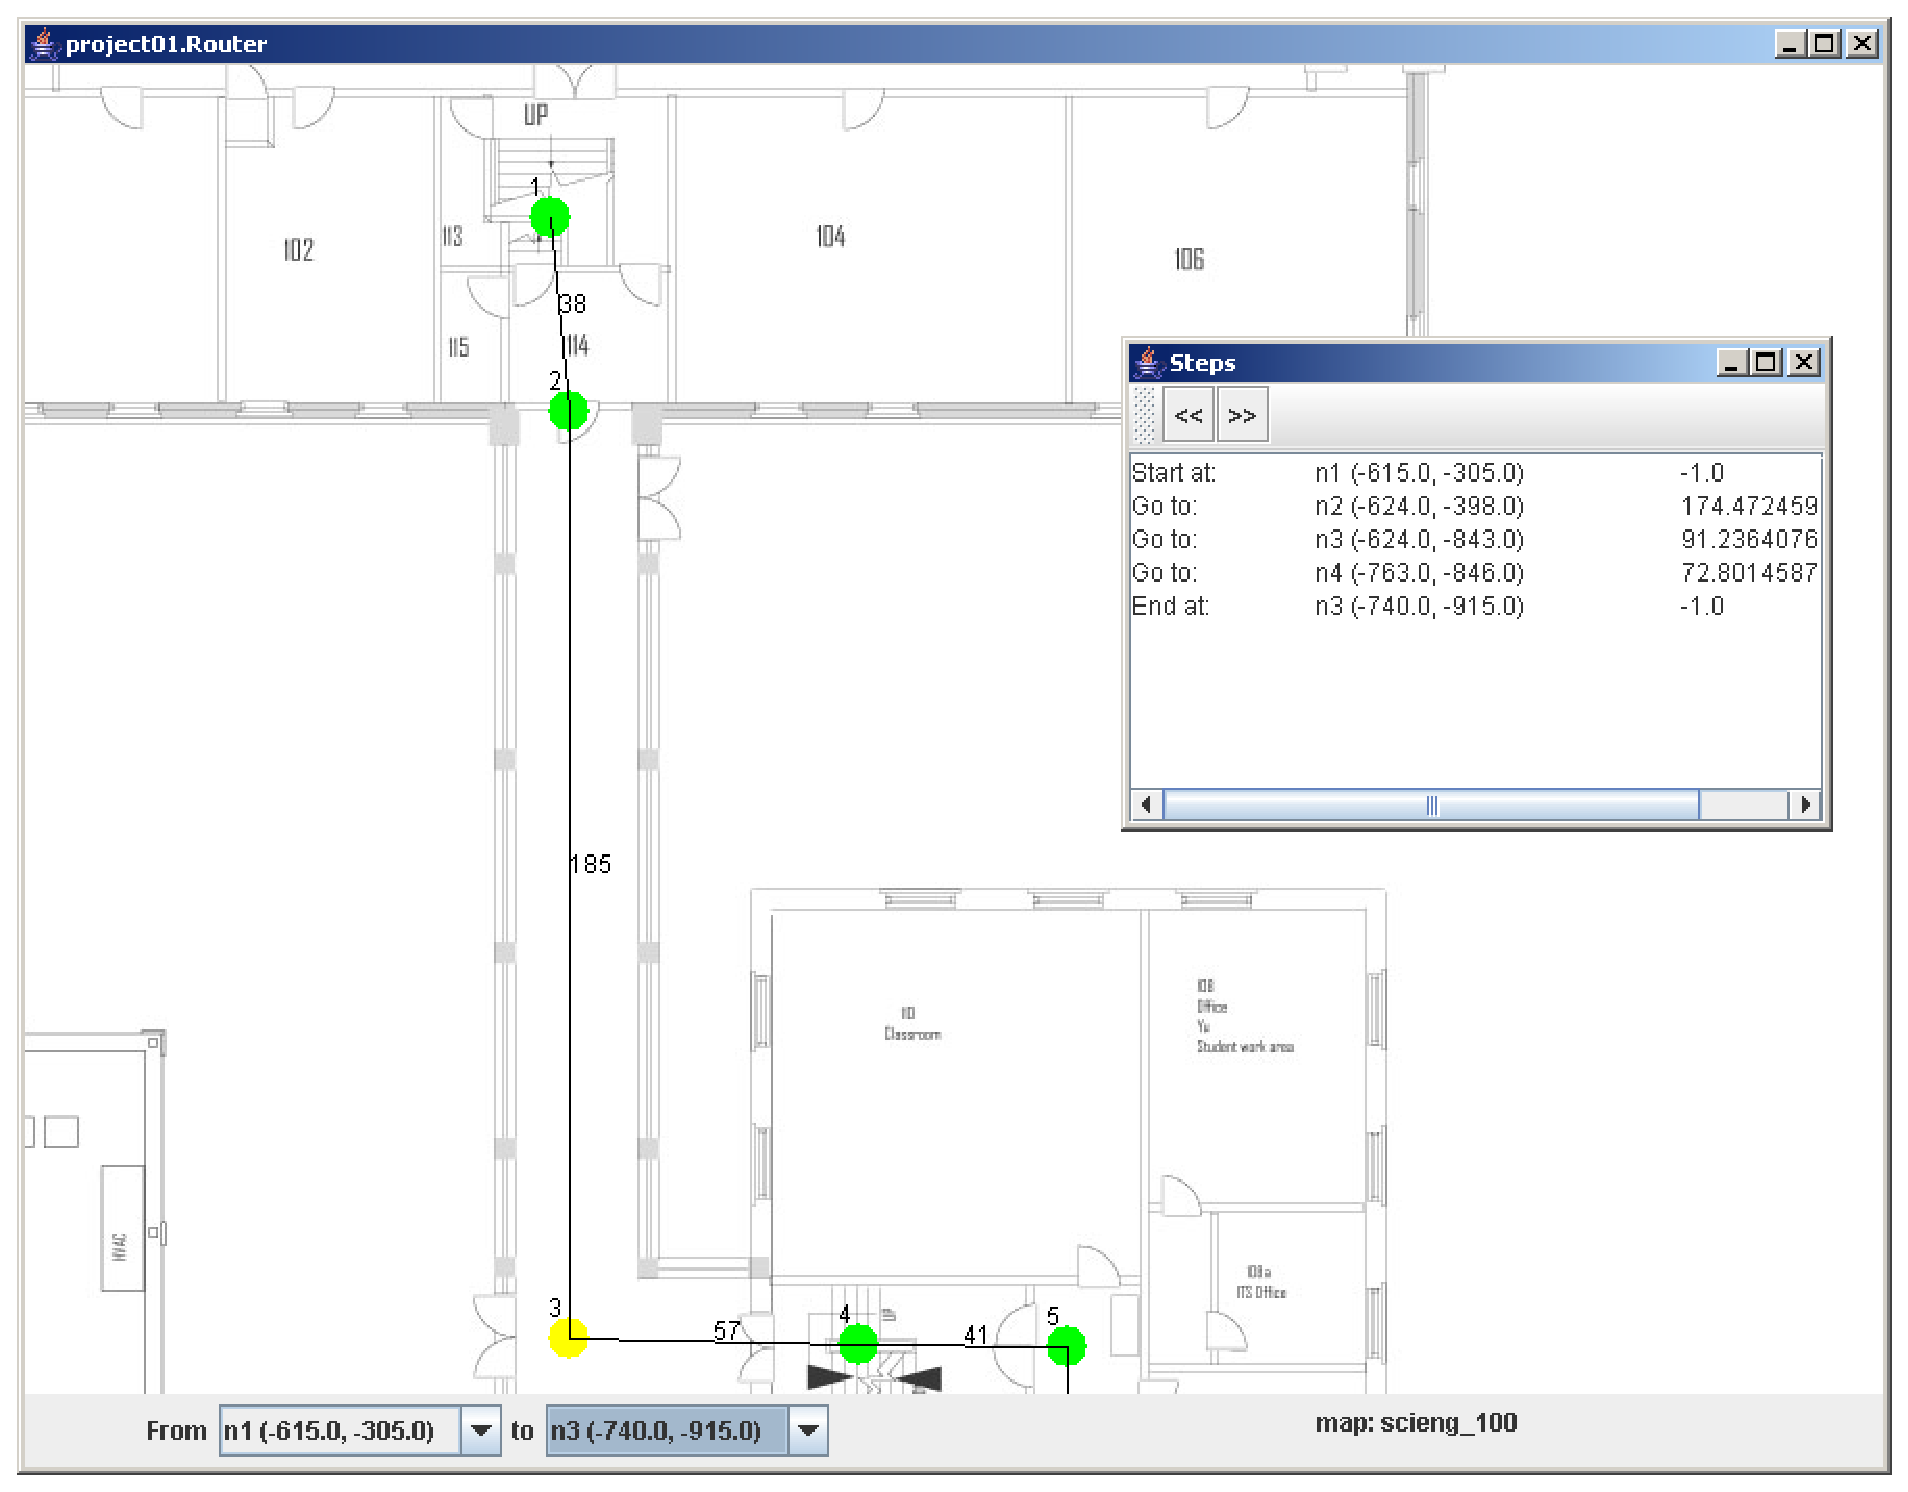
\includegraphics{images/pdf/router-screenshot}}
\end{center}
\caption{Router Mode}
\label{router-screenshot}
\end{figure}

\subsection{Editing}
Unlike \emph{Routing} mode, the nodes are not displayed immediately when the
program is opened. Therefore, the \emph{Load} button is used to load and
display the nodes for the respective map. Similarly, the \emph{Save} button is
used to store the node data in a file. Only one data file is stored per
map, and it assumes the same name as the map image file that it
corresponds to. The data file is stored in the root of the user's home
directory. On Unix-like platforms this is typically found in
\texttt{/home/username}, while on Windows NT-based machines this is found
in \texttt{$\backslash$Documents and Settings$\backslash$username}. A screen capture of
this mode is shown in Figure \ref{editor-screenshot-1}.

The map can be moved around on the screen using the sliders on the top
and left parts of the screen, or using click-and-drag, or using the
mouse scroll wheel. When the wheel is clicked, the map will pan about
the opposite axis.

A node can be created by double-clicking over the desired location. It
can be moved via click-and-drag. To modify the node's properties,
double-click it. The node's name can be changed in the properties window
that opens. If desired, the node can also be deleted through this
window.

To create edges, click-and-drag between two existing nodes. To delete
the edge or modify its distance, double-click either of the nodes that
it connects, go to the Edges tab, and select the correct edge.
\begin{figure}
\begin{center}
  \scalebox{0.5}[0.5]{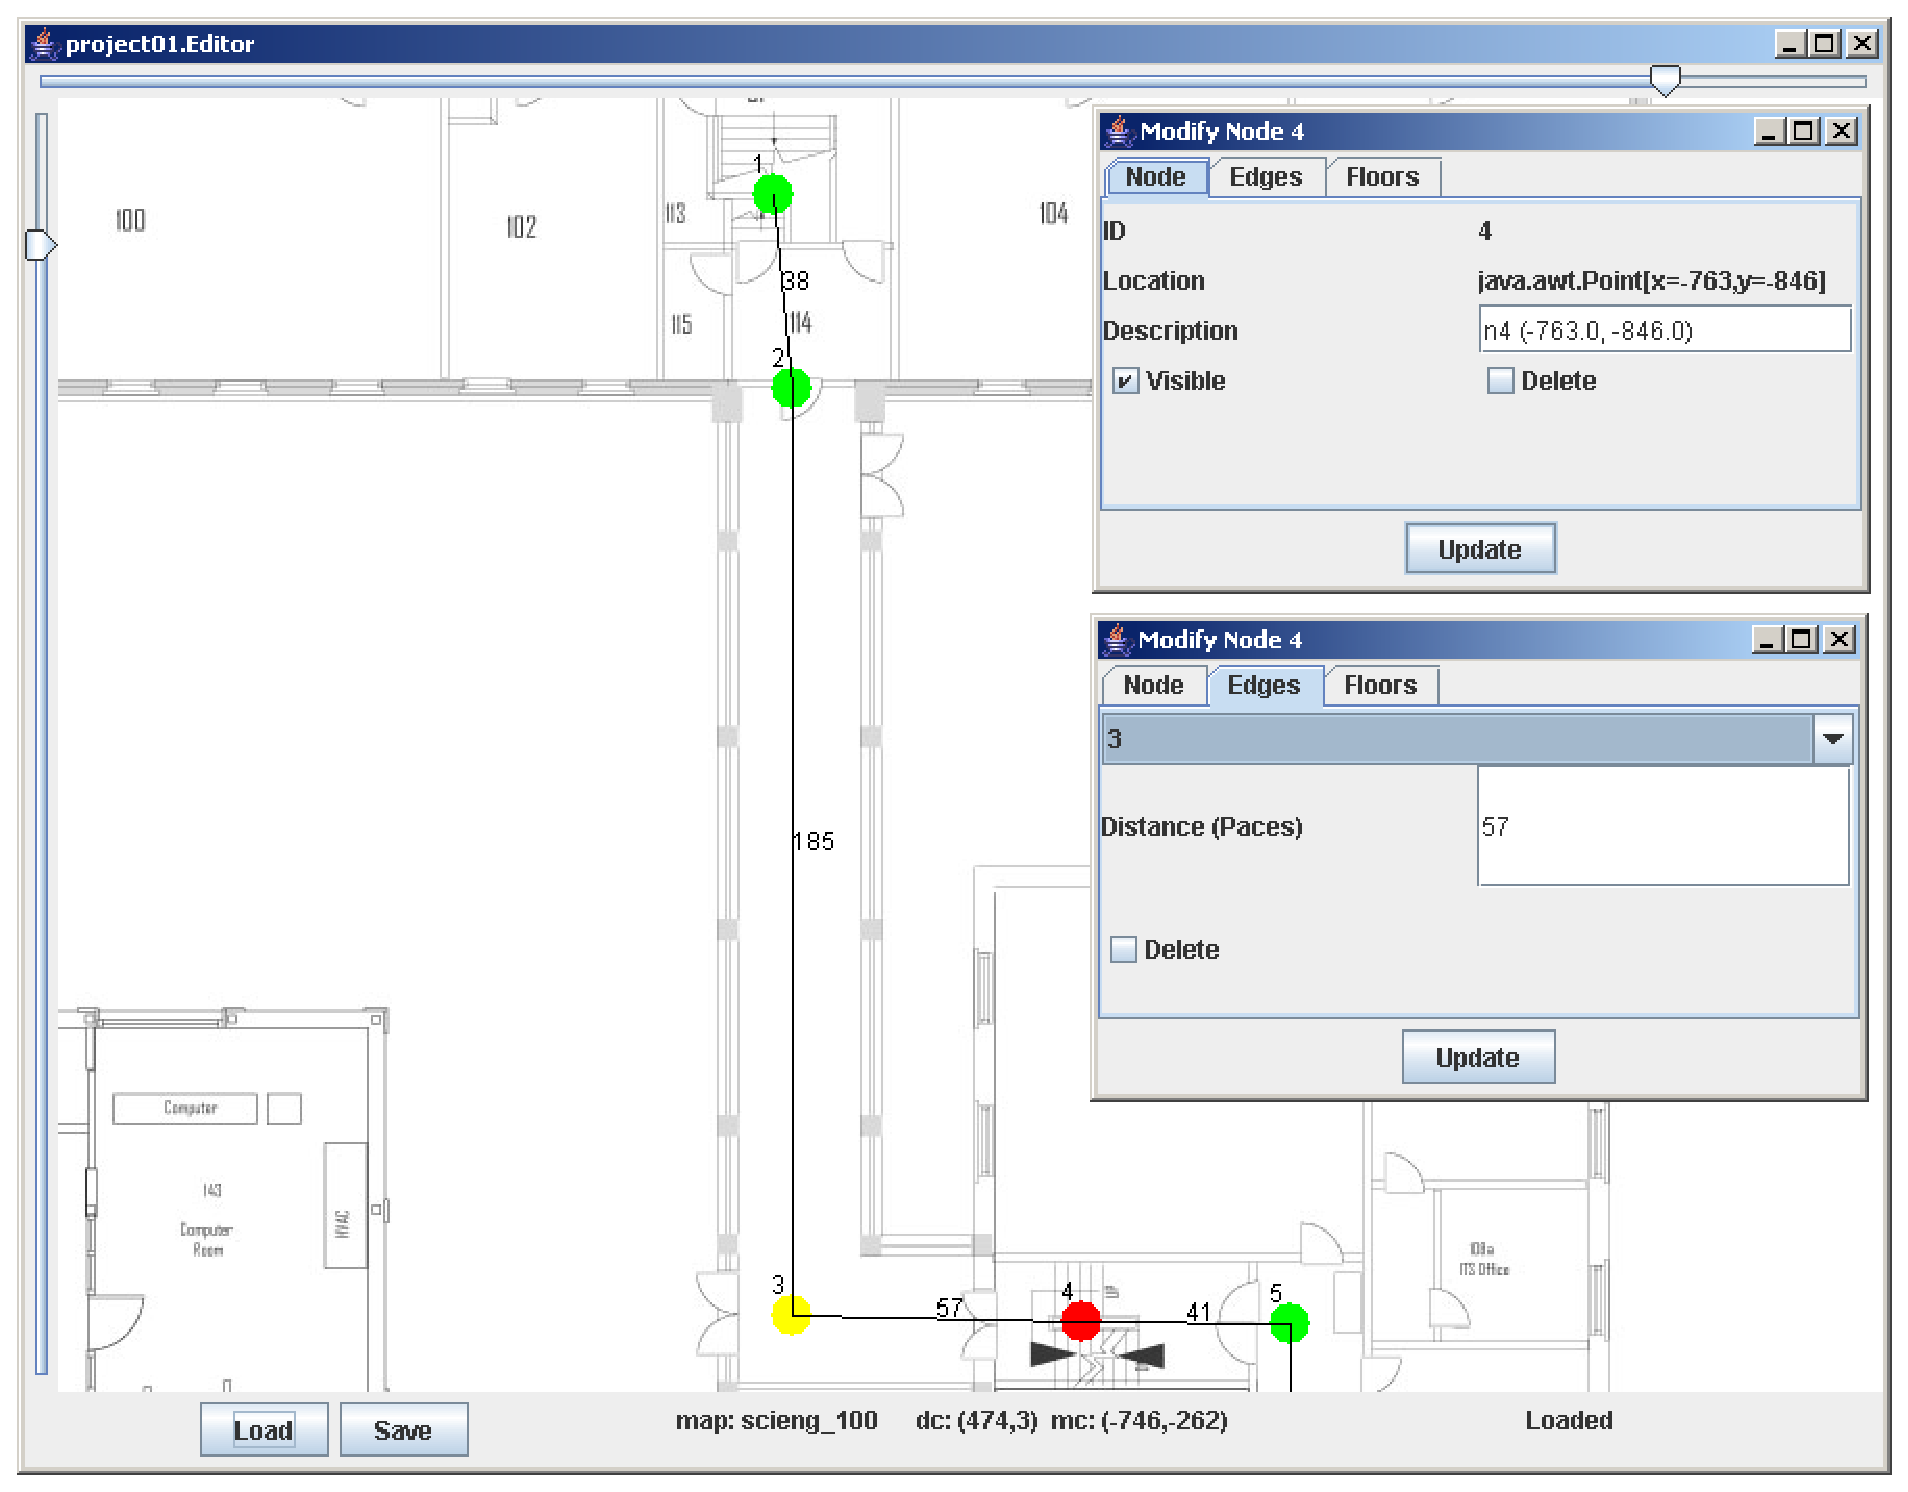
\includegraphics{images/pdf/editor-screenshot-1}}
\end{center}
\caption{Editor Mode}
\label{editor-screenshot-1}
\end{figure}

To create a floor link (i.e., represent a stairwell or elevator),
double-click the node at the correct stairwell, and go to the \emph{Floors}
tab. Select \emph{Links Floors} and click \emph{Add New Link}. Double-click the
correct corresponding node in the new window that opens. Click \emph{Add New
Link} again to set the link on the other corresponding floor. A screen
capture of the floor link feature in action is shown in
Figure \ref{editor-screenshot-2}.

\begin{figure}
\begin{center}
  \scalebox{0.5}[0.5]{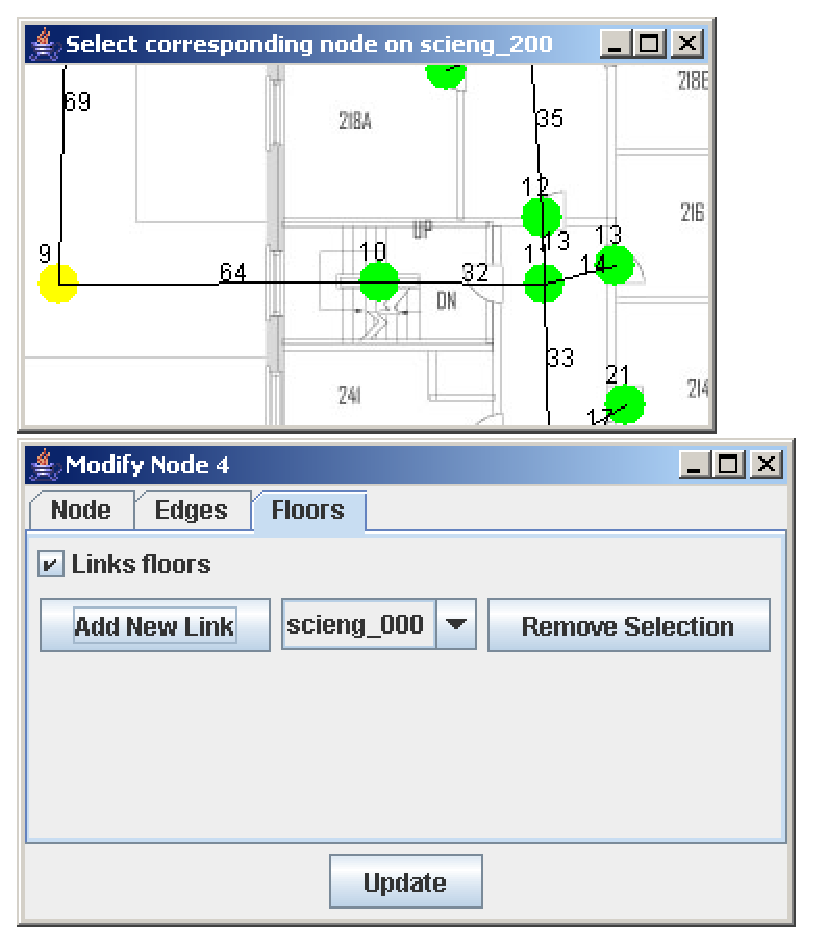
\includegraphics{images/pdf/editor-screenshot-2}}
\end{center}
\caption{Floor Linking in Editor Mode}
\label{editor-screenshot-2}
\end{figure}
 
\subsection{New Maps}
Every map image file must be in JPEG (\texttt{.jpg}) format, and begin with the
name ``map\_'' in the project's images directory. Since all maps are
stored within the JAR, when maps are added to the program they must be
included into the JAR file. The easiest way to do this is to simply add
the files into the correct directory, and recreate the JAR using ant.
Note that the map images must have print resolution of 96dpi. See section
\ref{bugs}.

\subsection{Development / Class Reference}
This software was developed using Java 1.5/JDK 5.0 Standard Edition with
the NetBeans 4.1 IDE. Please refer to the appendix for the source code.


\section{Known Bugs}
\label{bugs}

One of the goals of the project was to be able to provide the shortest
path between two locations. While this was achieved for any two
locations on a specific floor, as of this writing I have not yet proven
that the shortest route is also correctly obtained between two floors.
As mentioned above, within the \texttt{Dijkstra} class, 
\texttt{nearestFloorLink()}
returns the first floor-linking node found, but this may not actually be
the physically closest floor-link available. It may in fact actually be
in a non-optimal direction relative to the route as a whole.
Occasionally a floor link may not even be found, and currently this
causes the program to crash. I've also discovered that a stack overflow
occurs when going between three floors. I am working hard at fixing
these specific problems. Again, the first concern was to ensure that the
\texttt{Dijkstra} class could be used to work with multiple floors, and these
bugs in \texttt{nearestFloorLink()} will be fixed as soon as possible.

A requirement for the returned directions is that they are
``step-by-step''. While the program currently does this, it would be
more useful to provide turning directions (i.e., left and right) when
turning is required. It would also be more usable if points along a
straight path were not returned, i.e., points between the beginning and
end of a hallway were not presented in the directions if the user was
required to walk the complete length of the hallway. Both of these
problems can be resolved using an angle-based approach, where the angle
determined between three points describes the direction that the user
must follow. At the time of this writing, this directions enhancement is
in the process of being completed.

To correctly determine the physical distance between two points, both
the physical dots-per-inch resolution and the screen resolution need to
be determined. Unfortunately, not all JPEGs have dpi information listed
in their JFIF metadata, and when they do, it's not always in the same
field. Two different techniques were used to extract dpi information
from the maps used, and both failed (\texttt{ImageInfo} class from
\url{schmidt.devlib.org} and Sun's \texttt{JPEGImageDecoder} class).
Therefore, the dpi
for the map files was hardcoded into \texttt{MapComponent}. Eventually, a method
should be provided such that the program can dynamically determine dpi
of any map image, so that different print resolutions can be used.

In \emph{Router} mode, the map loaded via the commandline arguments must
contain the point of the desired starting location. If a point on a
different map is selected, then the program will not function
correctly.

Finally, the applet functionality needs to be fixed. Currently the
program does not execute correctly when invoked as an applet.


\section{Discussion, Conclusions, Recommendations}

Since I became aware of MapQuest, I had always wondered how driving
directions systems worked. It seemed pretty phenomenal to be able to
instantaneously obtain directions to anywhere that I wanted to go.
Considering the complexity of the Science and Engineering building,
it seemed like it would be useful to be able to have a similar 
directions service for locations on Union's campus.
Creating my own program to do this, however, seemed
unrealistic---some companies are entirely based around on collecting
geographic data and producing GIS technology. John and David helped me
understand some of the core concepts behind the technology, so that I
could adapt it to our campus buildings. By using existing floor plans, I
didn't have to worry about creating my own geographical data. This
allowed me to focus strictly on the shortest path problem (using
Dijkstra's algorithm) and creating a usable graphical interface.
It was still quite a challenging project,
and there was much I needed to learn through doing.

I'd never had much exposure to GUI development before, and I'd never
done any graphics programming at all. Fortunately, Sun provides great
documentation for Java. I hadn't yet taken the CSC-140/Data Structures
course at Union, so many complex data structures in the program were
represented with linked lists. This stemmed from the recommendation to
use linked lists as a basis for the graph object. Since they worked so
well for the graph object, I ended up using them all over the place. At
the time, I wasn't aware of the other possible built-in data structures,
and looking back on it now, there are many places in the program that
other data types would have been more appropriate. Thanks to Java's
inheritance, polymorphism and generics, it shouldn't be too hard to go
back and make these updates. Had I taken CSC-140 just one term earlier,
I would have been able to write code that better reflected some of the
data that I needed to represent.

Solely using linked lists was the least of my worries during
development, though. There were quite a few obstacles that we hadn't
considered during planning. Some of the highlights included finding out
how to draw the map image onto the screen, dealing with multiple
coordinate systems, implementing the Dijkstra algorithm correctly, and
reworking other internal functionality issues. For the map drawing,
Aaron Cass suggested using a custom \texttt{JComponent}
(\texttt{MapComponent}), which worked out very well. The AWT 
drawing tools naturally drew the nodes and
edges right over the image data, and as a \texttt{JComponent}, it was simple
integrating it into Swing frames.

The separate coordinate systems relating the mouse to the map were a bit
of a challenge, considering that the map coordinates make little sense
without a clear understanding of how Java handles components.
Implementing Dijkstra's algorithm took much longer than I expected. The
first attempt yielded working code, but it was extremely difficult to
follow and didn't accurately reflect the algorithm's definition. The
current Dijkstra class uses a much cleaner approach.

By the time I got to linking floors together, I realized that including
\texttt{NodeManager} within \texttt{MapComponent} may not have been the
best design choice. Since they're so closely related, it does make
sense to do this, however, when only the nodes need to be loaded,
the memory consumed by the base map goes to waste. When linking floors,
the data of both floors must be loaded, linked correctly, and saved.
Considering Java's limited
heap, the size of these map images, and the image-loading overhead, I
found that loading two floors simultaneously lead to out-of-memory
errors. Though it may have been better to separate the NodeManager from
the start, too much of the program was already dependent on the
all-in-one approach. Therefore, I added the \texttt{initMap()} method to
MapManager to indicate whether or not it should load the corresponding
map image. This has shown me how important top-down design is, and how
planning ahead really makes a difference. 

I'm still working on problems as mentioned in the previous section,
related to directional advice using angles, and correctly locating the
best stairwell/elevator for travel between floors on a route. In the
future I would like to create a more aesthetically-pleasing interface,
and expand the project to include both outdoor and indoor locations on
campus.

This was a really fun project! I learned quite a bit about graphics and
GUI programming, and shortest-path algorithms. ``Getting it right'' took
much revising, and I understand now more than ever before why well-
structured code is so important. Finally, I pleased that the program can
be used immediately by Union College to help guests and new students
navigate our buildings.


\pagestyle{plain} %headings
\bibliographystyle{/home/users/08/melnicki/texmf/tex/latex/apacite/apacite}
\bibliography{gpreport}
\nocite{*}

\newpage
\pagestyle{fancy} %headings
\appendix
\section{Source Code}

This code is free for academic use at Union College, but credit must be
given if it is incorporated into other projects. It cannot be used in
products to be sold without the author's written consent.

\singlespacing
\begin{spacing}{0.7}
\tiny


\subsection{Console.java}
\begin{lgrind}
\input src/Console.java.tex
\end{lgrind}

\subsection{Dijkstra.java}
\begin{lgrind}
\input src/Dijkstra.java.tex
\end{lgrind}

\subsection{DirectionsFrame.java}
\begin{lgrind}
\input src/DirectionsFrame.java.tex
\end{lgrind}

\subsection{EdgeItem.java}
\begin{lgrind}
\input src/EdgeItem.java.tex
\end{lgrind}

\subsection{Editor.java}
\begin{lgrind}
\input src/Editor.java.tex
\end{lgrind}

\subsection{Errors.java}
\begin{lgrind}
\input src/Errors.java.tex
\end{lgrind}

\subsection{FloorLinker.java}
\begin{lgrind}
\input src/FloorLinker.java.tex
\end{lgrind}

\subsection{Main.java}
\begin{lgrind}
\input src/Main.java.tex
\end{lgrind}

\subsection{MapComponent.java}
\begin{lgrind}
\input src/MapComponent.java.tex
\end{lgrind}

\subsection{MapItem.java}
\begin{lgrind}
\input src/MapItem.java.tex
\end{lgrind}

\subsection{NodeEditor.java}
\begin{lgrind}
\input src/NodeEditor.java.tex
\end{lgrind}

\subsection{NodeItem.java}
\begin{lgrind}
\input src/NodeItem.java.tex
\end{lgrind}

\subsection{Router.java}
\begin{lgrind}
\input src/Router.java.tex
\end{lgrind}

\subsection{Utility.java}
\begin{lgrind}
\input src/Utility.java.tex
\end{lgrind}



\normalsize
\end{spacing}
\doublespacing


\end{document}
